\section{Zielsetzung}

In diesem Versuch sollen die verschiedenen Schwingungsmodi gekoppelter Pendel untersucht werden.
Dabei werden die Schwingungs- und Schwebungsdauern von gleichsinniger,- gegensinniger und gekoppelter Schwingung gemessen.

\section{Theoretische Grundlagen}

Bei einem schwingendem Pendel wirkt die Gravitationskraft $\vec{F_g}=m \vec{g} $ der Bewegung entgegen, wobei $m$ die Masse des Pendels und $g$ die Gravitationsbeschleunigung ist.\\
Dadurch wirkt auf das Pendel ein Drehmoment von $M= D_p\phi$,  mit $\phi$ als Auslenkwinkel und $D_p$ als die Winkelrichtgröße.\\
Für die Bewegung des Teilchens lässt sich dann unter der Kleinwinkelnäherung folgende Differentialgleichung herleiten:
\begin{equation*}
    J \ddot{\phi} + D_p \phi=0
\end{equation*}
Dies ist die Differentialgleichung des harmonischen Oszillators. Lösen führt zu einer Frequenz der Bewegung von $\omega= \sqrt{\frac{D_p}{J}}=\sqrt{\frac{g}{l}}$.\\
Die Frequenz ist also für kleine Winkel unabhängig vom Auslenkwinkel.\\\\

\noindent
Nun sollen aber nicht nur einfache Schwingungen der Pendel untersucht werden sondern auch gekoppelte.\\
Dafür wird noch ein zusätzlicher Drehmoment-Term bei beiden Pendeln ergänzt, der in Abhängigkeit der Differenz der Winkel voneinander steht.\\
Dieser lautet dann $M_1=D_F (\phi_2 -\phi_1)$ beziehungsweise $M_1=-M_2$.
Daraus ergibt sich dann folgendes gekoppeltes Differentialgleichungssystem:
\begin{align*}
    J \ddot{\phi_1} + D_p \phi_1 & D_F (\phi_2 -\phi_1)\\
    J \ddot{\phi_2} + D_p \phi_2 & D_F (\phi_1 -\phi_2)
\end{align*}
Durch geeignete Wahl der Winkel lässt sich das Differentialgleichungssystem entkoppeln und als Überlagerung zweier Eigenschwingungen mit Kreisfrequenzen $\omega_1$ und $\omega_2$ lösen.\\
Die im folgenden besprochenen Fallunterscheidungen können das System mit richtiger Wahl der Anfangsbedingungen lösen.

\newpage
\begin{itemize}
    \item {\Large Gleichsinnige Schwingung\\}{
        \begin{figure}[H]
            \centering
            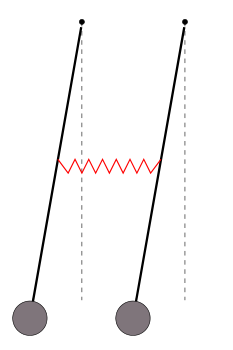
\includegraphics[width=0.2\textwidth]{latex/images/schwing1.PNG}
            \caption{Die schematische Abbildung einer gleichsinnigen gekoppelten Schwingung\protect \cite{V106}.}
            \label{img:1}
        \end{figure}
        \noindent
        Für den gleichsinnigen Fall lässt sich das Differentialgleichungssystem lösen mit der Anfangsbedingung $\alpha_1 = \alpha_2$.\\
        Abbildung \ref{img:1} stellt diesen Fall dar.\\
        Bei diesem Fall übt die Kopplung keine Kraft aus. 
        Es ergibt sich also als Lösung für beide Pendel einfach der ungekoppelte klassische Fall.\\
        Aus der Kreisfrequenz $\omega=\sqrt{\frac{g}{l}}$ lässt sich über $T=\frac{2 \pi}{\omega}$ die Schwingungsdauer $T=2 \pi \sqrt{\frac{l}{g}}$ bestimmen.\\
    }
    \item {\Large Gegensinnige Schwingung\\}{
        \begin{figure}[H]
            \centering
            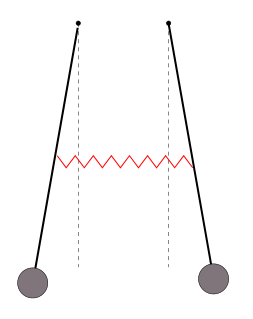
\includegraphics[width=0.2\textwidth]{latex/images/schwing2.PNG}
            \caption{Die schematische Abbildung einer gegensinnigen gekoppelten Schwingung\protect \cite{V106}.}
            \label{img:2}
        \end{figure}
        \noindent Die Anfangsbedingung für den gegensinnigen Fall ist $\alpha_1 = -\alpha_2$.\\
        Grafisch dargestellt ist dies in Abbildung \ref{img:2}.
        Hier wirkt die Kraft der Kopplung der Bewegung entgegen und bremst diese somit ab.
        Die Schwingungsfrequenz ergibt sich hier zu $\omega=\sqrt{\frac{g}{l}+\frac{2 \symup{K}}{l}}$ mit der Kopplungskonstante $\symup{K}$.\\
        Damit ist dann die Periodendauer $T=2 \pi \sqrt{\frac{l}{g}+\frac{l}{2 \symup{K}}} $.\\
        }

    \item {\Large Gekoppelte Schwingung\\}{
        \begin{figure}[H]
            \centering
            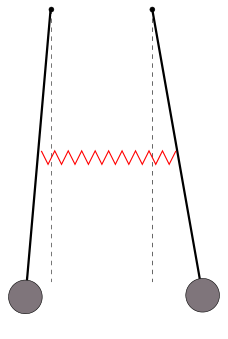
\includegraphics[width=0.2\textwidth]{latex/images/schwing3.PNG}
            \caption{Die schematische Abbildung einer gegensinnigen gekoppelten Schwingung\protect \cite{V106}.}
            \label{img:3}
        \end{figure}
        \noindent In diesem Fall befindet sich eines der gekoppelten Pendel in Ruhe und das andere wird ausgelenkt.
        Die Anfangsbedingungen ergeben sich also zu $\alpha_1=0$ und $\alpha_2 \neq 0$.\\
        Hier regt das schwingende Pendel das ruhende zum Schwingen an. Dabei überträgt es seine Energie und verliert dadurch an Amplitude.\\
        Dieser Vorgang setzt sich fort bis das Pendel komplett in Ruhe ist und seine gesamte Energie übertragen hat. Nun beginnt das jetzt ruhende Pendel angeregt zu werden.\\
        Der Zeitraum zwischen zwei identischen Zuständen eines Pendels wird Schwebung genannt. Ihre charakteristischen Größen sind:
        \begin{align*}
            T&=\frac{T_+ \cdot T_-}{T_+ - T_-} \\
            \omega_s&= \omega_+ -\omega_-
        \end{align*} 
        Alle mit \enquote*{+} gekennzeichneten Größen beziehen sich dabi auf die gleichsinnige Schwingung und alle mit \enquote*{-} gekennzeichneten auf die gegensinnige.\\
        Zusätzlich kann mit diesen Definitionen auch die zuvor erwähnte Kopplungskonstante $\symup{K}$ definiert werden.\\
        Diese ist dann nämlich:
        \begin{equation*}
            \symup{K}=\frac{T_+ - T_-}{T_+ + T_-}=\frac{\omega_+ -\omega_-}{\omega_+ + \omega_-}
        \end{equation*}

        
        }
\end{itemize}




